\documentclass[conference]{IEEEtran}
\IEEEoverridecommandlockouts
\usepackage{cite}
\usepackage{amsmath,amssymb,amsfonts}
\usepackage{algorithmic}
\usepackage{graphicx}
\usepackage{textcomp}
\usepackage{xcolor}
\usepackage{booktabs}
\usepackage{url}
\graphicspath{{figures/}}
\def\BibTeX{{\rm B\kern-.05em{\sc i\kern-.025em b}\kern-.08em
    T\kern-.1667em\lower.7ex\hbox{E}\kern-.125emX}}

\begin{document}

\title{SENTINEL: Organ-System Decomposition for Robust and Interpretable
Early Warning of Sepsis in the ICU}

\author{\IEEEauthorblockN{Anonymous Author(s)}
\IEEEauthorblockA{\textit{Affiliation} \\
City, Country \\
email}
}

\maketitle

\begin{abstract}
Deep models for ICU sepsis early warning are accurate but opaque, brittle when
inputs are missing, and require centralizing sensitive data. We ask whether
decomposing the patient into six organ-system agents aligned with the Sequential
Organ Failure Assessment (SOFA) score buys robustness, interpretability, and
privacy without sacrificing discrimination. On a MIMIC-IV cohort of 80,248 ICU
stays, the organ-decomposed model matches or beats a monolithic deep model on the
area under the precision--recall curve (AUPRC 0.257 vs.\ 0.205 on the internal
test set), and is markedly more robust to a missing organ signal: blinding any one
organ at test time costs the decomposed model a mean of 0.001 AUPRC versus 0.03--0.05
for the monolithic model. A controlled experiment---a six-member ensemble on the
joint feature vector with the identical max-combine rule---degrades exactly like the
monolithic model, establishing that the robustness comes from \emph{organ
decomposition}, not ensembling. The decomposition is interpretable (per-organ risk
attribution) and trainable across non-IID care-unit ``sites'' via federated
averaging at a quantified utility cost. In contrast, we find---and report
plainly---that adding cooperative multi-agent reinforcement learning yields no
benefit: a centralized critic (MAPPO) is statistically indistinguishable from
independent learners (IPPO), and a utility-trained policy is a far weaker
discriminator than supervision. We argue this null is principled: because alerting
does not perturb the patient, the observation trajectory is exogenous and the
cooperative coupling that motivates a centralized critic is absent. All numbers are
reported with bootstrap confidence intervals on internal and external splits; the
pipeline and analysis are fully reproducible.
\end{abstract}

\begin{IEEEkeywords}
sepsis, early warning, MIMIC-IV, interpretability, robustness, multi-agent
reinforcement learning, federated learning
\end{IEEEkeywords}

\section{Introduction}
Sepsis is a leading cause of in-hospital mortality, and early recognition improves
outcomes. Machine-learning early-warning systems are increasingly deployed, but
three concerns limit their clinical trust. First, the strongest models are
\emph{black boxes}: a single risk score offers no account of \emph{which} organ
system is deteriorating. Second, they are \emph{brittle}: ICU data are intermittently
missing, and a model trained on the full feature vector can fail silently when a
signal goes dark. Third, training typically requires \emph{centralizing} patient
records across institutions, which is often legally infeasible. A widely deployed
proprietary sepsis model was recently shown to underperform on external validation,
in part by latching onto clinician \emph{ordering behavior} rather than physiology
\cite{wong2021epic}---a cautionary tale for the whole approach.

We study a structural alternative: decompose the patient into six organ-system
agents aligned with the SOFA score \cite{vincent1996sofa}
(respiratory, coagulation, hepatic, cardiovascular, neurologic, renal), each
observing only its own subsystem, and combine their organ-specific onset risks. The
\emph{escalation action} is alerting (maintain / watch / escalate), never treatment
dosing---a deliberate choice that keeps evaluation valid and sidesteps the
off-policy-evaluation pitfalls of offline reinforcement learning (RL) for treatment
\cite{gottesman2019guidelines,komorowski2018aiclinician}.

Our contributions, each tied to a controlled result:
\begin{itemize}
  \item \textbf{Decomposition matches/beats a monolithic deep model} on AUPRC, with
        bootstrap confidence intervals, on internal and external splits.
  \item \textbf{Decomposition---not ensembling---confers missing-signal robustness},
        established by a joint-feature ensemble control.
  \item \textbf{Interpretability} via per-organ risk attribution, demonstrated in a
        replay dashboard.
  \item \textbf{Federated feasibility at a quantified privacy cost} across non-IID
        care units.
  \item \textbf{A principled null for cooperative coordination}: MAPPO $\approx$ IPPO,
        explained by the exogenous-dynamics structure of alerting.
\end{itemize}
We report every result that weakened a claim rather than hiding it.

\section{Related Work}
Rule-based early-warning scores such as NEWS \cite{rcp2017news2} are interpretable
but weak discriminators. Supervised sepsis predictors on MIMIC
\cite{henry2015trewscore,johnson2023mimiciv} are stronger but monolithic and
opaque, and external validation can expose shortcut learning \cite{wong2021epic}.
Multi-agent RL has been explored for healthcare, but cooperative methods---MAPPO
\cite{yu2022mappo}, QMIX \cite{rashid2018qmix}, MADDPG \cite{lowe2017maddpg}---are
motivated by agents perturbing a shared environment; IPPO \cite{dewitt2020ippo} is
the natural control isolating the value of a centralized critic. Federated averaging
\cite{mcmahan2017fedavg} enables training without pooling data, but non-IID clients
degrade utility \cite{zhao2018noniid}. Fairness and shortcut concerns in clinical ML
are well documented \cite{obermeyer2019bias}. We bring these threads together with
an emphasis on \emph{controlled} attribution of where decomposition helps.

\section{Methods}
\subsection{Cohort and Sepsis-3 labels}
From MIMIC-IV v3.1 \cite{johnson2023mimiciv} we build a cohort of first ICU stays
(adults 18--89, length of stay $\geq 6$\,h; 80{,}248 stays). We reimplement the
Sepsis-3 criteria \cite{singer2016sepsis3,seymour2016assessment}, cross-checked
against the MIMIC code repository \cite{johnson2018mimiccode}: suspicion of
infection (antibiotic + culture within the standard window) co-occurring with an
acute rise in hourly SOFA. We use a \emph{dynamic baseline}---the acute rise is
measured against the patient's pre-suspicion admission SOFA---giving a prevalence of
37.4\% and, crucially, a clean \emph{three-way split}: positives are stays with
onset at least $H{=}6$\,h into the stay (8{,}763); stays that are septic earlier or
present-on-admission are \emph{excluded} from both classes; controls never meet
Sepsis-3. Derivations are validated by unit tests against hand-checked stays.

\subsection{Features and the exogenous-dynamics formulation}
Per organ we form hourly features (values, missingness masks, and measurement
indicators), with physiologic forward-fill and train-split-only normalization;
a room-air FiO$_2$ default and an SpO$_2$/FiO$_2$ surrogate \cite{rice2007sfratio}
address sparse blood gases. The decision process is a decentralized partially
observable problem: each organ agent sees its own subsystem plus minimal shared
context. Critically, \emph{alerting does not change the patient}, so the observation
trajectory is exogenous: the reward of any action sequence is exactly computable from
the record. This removes the off-policy-evaluation problem entirely and frames the
learning as policy-gradient optimization of a non-differentiable clinical utility,
not decision-making under environment uncertainty.

\subsection{Models}
\textbf{SENTINEL (organ-decomposed).} Six per-organ GRU \emph{risk heads} are trained
by supervision; the team onset risk is their max-combine---the score compared on
AUPRC, and the source of structural robustness (blinding one organ disables one of
six heads). \textbf{Alarm policy.} A small policy over the organ risks and the
alert history is trained with PPO \cite{schulman2017ppo} and GAE
\cite{schulman2016gae} on a ramped early-warning utility (lead-time bonus, miss
penalty, false-alarm and per-alarm-event costs). \textbf{Cooperative variants.}
MAPPO uses a centralized critic over the joint state; IPPO uses per-organ critics---
the only difference, isolating coordination. \textbf{Federated.} We partition
training data by admitting care unit (genuinely non-IID; e.g.\ medical ICU $\sim$54\%
sepsis vs.\ neuro $\sim$16\%) and train a shared model by FedAvg \cite{mcmahan2017fedavg}
without pooling data, holding out one unit as an external site.

\section{Experimental Setup}
Splits are temporal by anchor-year group (train 2008--2016 / val 2017--2019 / test
2020--2022), with the cardiac-vascular ICU held out entirely as the external site.
Baselines: NEWS2 \cite{rcp2017news2}, XGBoost, and a monolithic GRU. The primary
metric is AUPRC (class imbalance $\approx$5\% positive hours) with 95\% bootstrap
confidence intervals resampled over \emph{stays}; we also report AUROC, the alert
lead time, and the alarm burden as distinct \emph{alarm events} per patient-day
(rising edge with a refractory window), with the operating threshold chosen on
validation at a fixed budget. Learned models use 3--5 seeds. Compute is a single
4\,GB GPU; all training is FP32.

\section{Results}
\subsection{Discrimination}
Table~\ref{tab:disc} and Fig.~\ref{fig:disc} show the organ-decomposed model
matching or beating the monolithic GRU---AUPRC 0.257 vs.\ 0.205 on internal test
(confidence intervals barely overlap), comparable externally---and roughly doubling
XGBoost. The utility-trained MAPPO/IPPO policies are weak discriminators
($\sim$0.06), as expected when optimizing alarm utility rather than the label.

\begin{table}[t]
\caption{Discrimination (AUPRC; 95\% CI). No-skill: 0.049 / 0.057.}
\label{tab:disc}
\centering\small
\begin{tabular}{lcc}
\toprule
Model & internal test & external (CVICU) \\
\midrule
NEWS2 & 0.066 & 0.051 \\
XGBoost & 0.115 & 0.242 \\
GRU-single (monolithic) & 0.205 & \textbf{0.283} \\
JointEnsemble-6 (control) & 0.202 & 0.283 \\
\textbf{SENTINEL (organ-decomposed)} & \textbf{0.257} & 0.265 \\
SENTINEL-MAPPO $\approx$ IPPO & 0.063 & 0.051 \\
\bottomrule
\end{tabular}
\end{table}

\begin{figure}[t]
\centering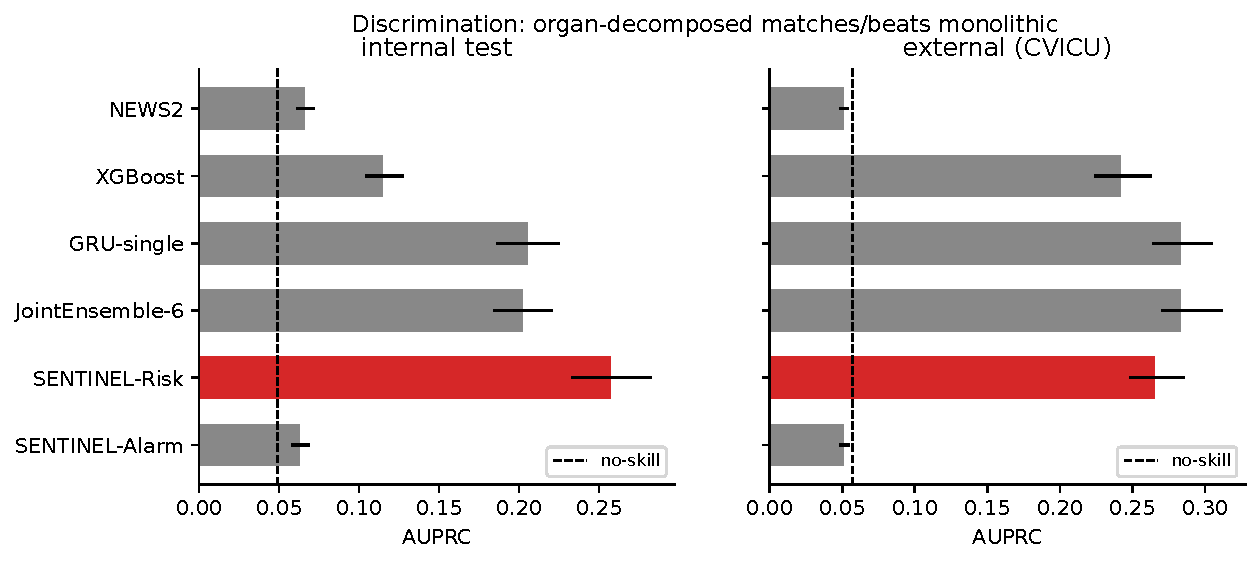
\includegraphics[width=\columnwidth]{fig_discrimination.pdf}
\caption{AUPRC by model with 95\% CIs and the no-skill line. Organ decomposition
(red) matches/beats the monolithic deep model.}
\label{fig:disc}
\end{figure}

\subsection{Missing-signal robustness, controlled}
Fig.~\ref{fig:rob} is the central result. Blinding any one organ's inputs at test
time costs the decomposed model a mean of $-0.001$/$-0.002$ AUPRC (test/external),
versus $-0.028$/$-0.041$ for the monolithic GRU. The control---\textsc{JointEnsemble-6},
six GRUs on the \emph{joint} vector with the same max-combine---degrades like the
monolithic model ($-0.030$/$-0.056$), and at full inputs is no stronger than it
(0.202 vs.\ 0.199). Thus the robustness, and the discrimination gain, come from
\emph{organ decomposition}, not from ensembling. The starkest case: with the
cardiovascular organ blinded on the external unit, the decomposed model holds 0.273
while both the joint ensemble (0.173) and the monolithic model (0.176) collapse.

\begin{figure}[t]
\centering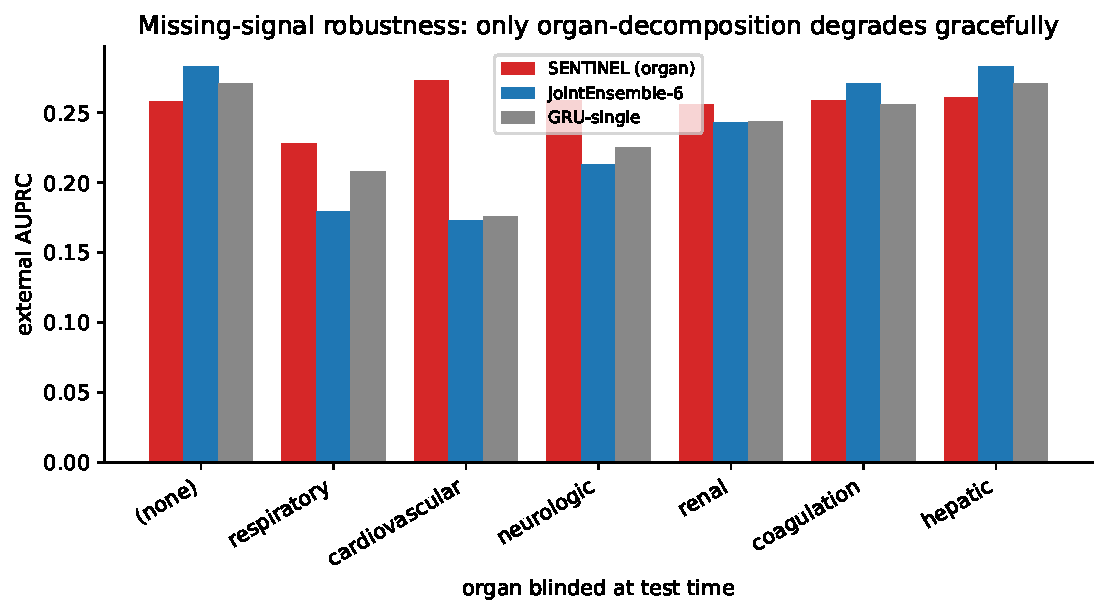
\includegraphics[width=\columnwidth]{fig_robustness.pdf}
\caption{External AUPRC as each organ is blinded. Only organ-decomposition (red)
degrades gracefully; the ensembling control collapses with the monolithic model.}
\label{fig:rob}
\end{figure}

\subsection{What the non-physiology signal is}
Fig.~\ref{fig:abl} decomposes the gap between physiology-only and full inputs. With
tight confidence intervals on the full cohort, dropping the measurement/ordering
channels costs essentially nothing ($-0.002$, not significant), while dropping the
temporal prior costs the rest ($-0.07$ to $-0.08$). The non-physiology signal here is
a benign timing prior, \emph{not} the clinician-ordering shortcut that has undermined
deployed models \cite{wong2021epic}.

\begin{figure}[t]
\centering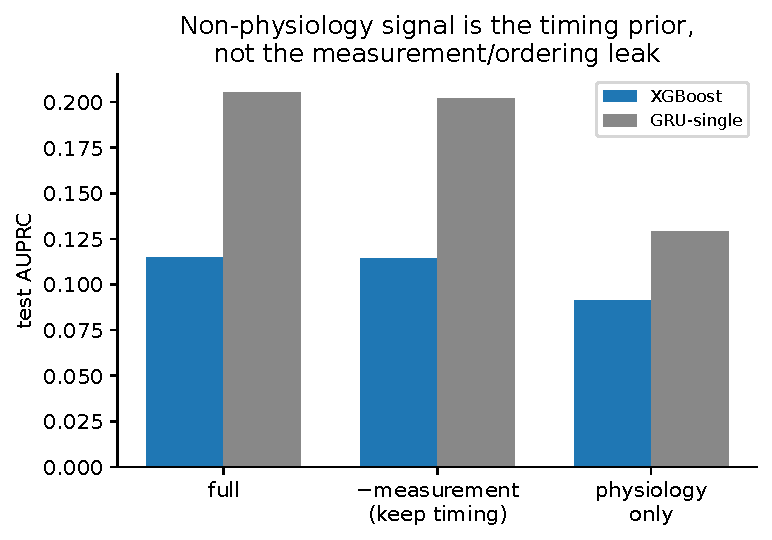
\includegraphics[width=0.86\columnwidth]{fig_ablation.pdf}
\caption{Ablation: the non-physiology signal is the timing prior, not the
measurement/ordering leak.}
\label{fig:abl}
\end{figure}

\subsection{Coordination is a measured null}
SENTINEL-MAPPO and SENTINEL-IPPO are statistically indistinguishable on every split
(e.g.\ test AUPRC 0.063 vs.\ 0.066, overlapping CIs). Scaling training five-fold did
not move the policy's discrimination. We read this as principled rather than a
failure: under exogenous alerting dynamics no agent perturbs the environment, so the
only coupling is the shared reward and the max-combine, and a centralized critic has
nothing to coordinate. An action-history-conditioned actor variant matched the
observation-only policy, empirically justifying the simplification.

\subsection{Federated privacy cost}
Across eight non-IID care units, FedAvg reaches AUPRC 0.121 (test) / 0.237 (external)
versus 0.212 / 0.290 centralized---a real cost of $-0.091$ / $-0.052$, yet still well
above no-skill. Privacy-preserving training is feasible but not free when sites are
strongly non-IID \cite{zhao2018noniid}.

\section{Discussion}
The decomposition buys exactly what a monolithic model cannot: per-organ
attribution and a structural fallback when a signal is missing, at no discrimination
cost---indeed a gain. The cooperative-MARL machinery, by contrast, adds nothing here,
and we believe the exogenous-dynamics analysis explains why and generalizes to other
\emph{alerting} (as opposed to \emph{acting}) clinical tasks. The honest takeaway is
that \emph{structure}, not \emph{coordination}, is the useful inductive bias.

\section{Limitations}
Single-source data (MIMIC-IV); ``sites'' are simulated by care unit, not real
institutions; labels are retrospective and the escalation action is a proxy for real
clinical response. The internal test set has a few hundred positive episodes, so we
lean on the external split and CIs. The federated study uses a single shared model;
federating the organ heads is future work.

\section{Reproducibility and Ethics}
The pipeline is config-driven with fixed seeds; cohort, labels, features, training,
evaluation, and figures regenerate end-to-end, and unit tests cover the Sepsis-3
derivation, the reward, leakage, and the MARL gates. MIMIC-IV is credentialed under a
PhysioNet data-use agreement; no raw or derived row-level data is shared.

\section{Conclusion}
Organ-system decomposition gives an ICU early-warning model that matches or beats a
monolithic deep network, is uniquely robust to missing signals (a controlled result),
is interpretable, and is federatable at a measured cost---while cooperative
coordination, tested rigorously, provides no benefit. We argue for structure over
coordination in exogenous-dynamics clinical alerting.

\bibliographystyle{IEEEtran}
\bibliography{references}

\end{document}
